\section{Oscillatorer}
\textbf{HAREC a.\ref{HAREC.a.3.6}\label{myHAREC.a.3.6}}
\index{oscillator}
\label{oscillatorer}

\subsection{Alstring av svängningar}
Ordet \emph{oscillare} (lat.) har betydelsen svänga och den företeelse
eller anordning som skapar en svängning kallas oscillator. Vid alla
slags svängningar sker växelverkan mellan olika
energiformer. Svängningar förekommer i olika former. Det kan vara
vibrationer i en kropp, en pendel som svänger, rörelser i gaser och
vätskor, elektriska laddningar i en strömkrets o.s.v.

\subsubsection{Mekanisk pendel}

\begin{figure}
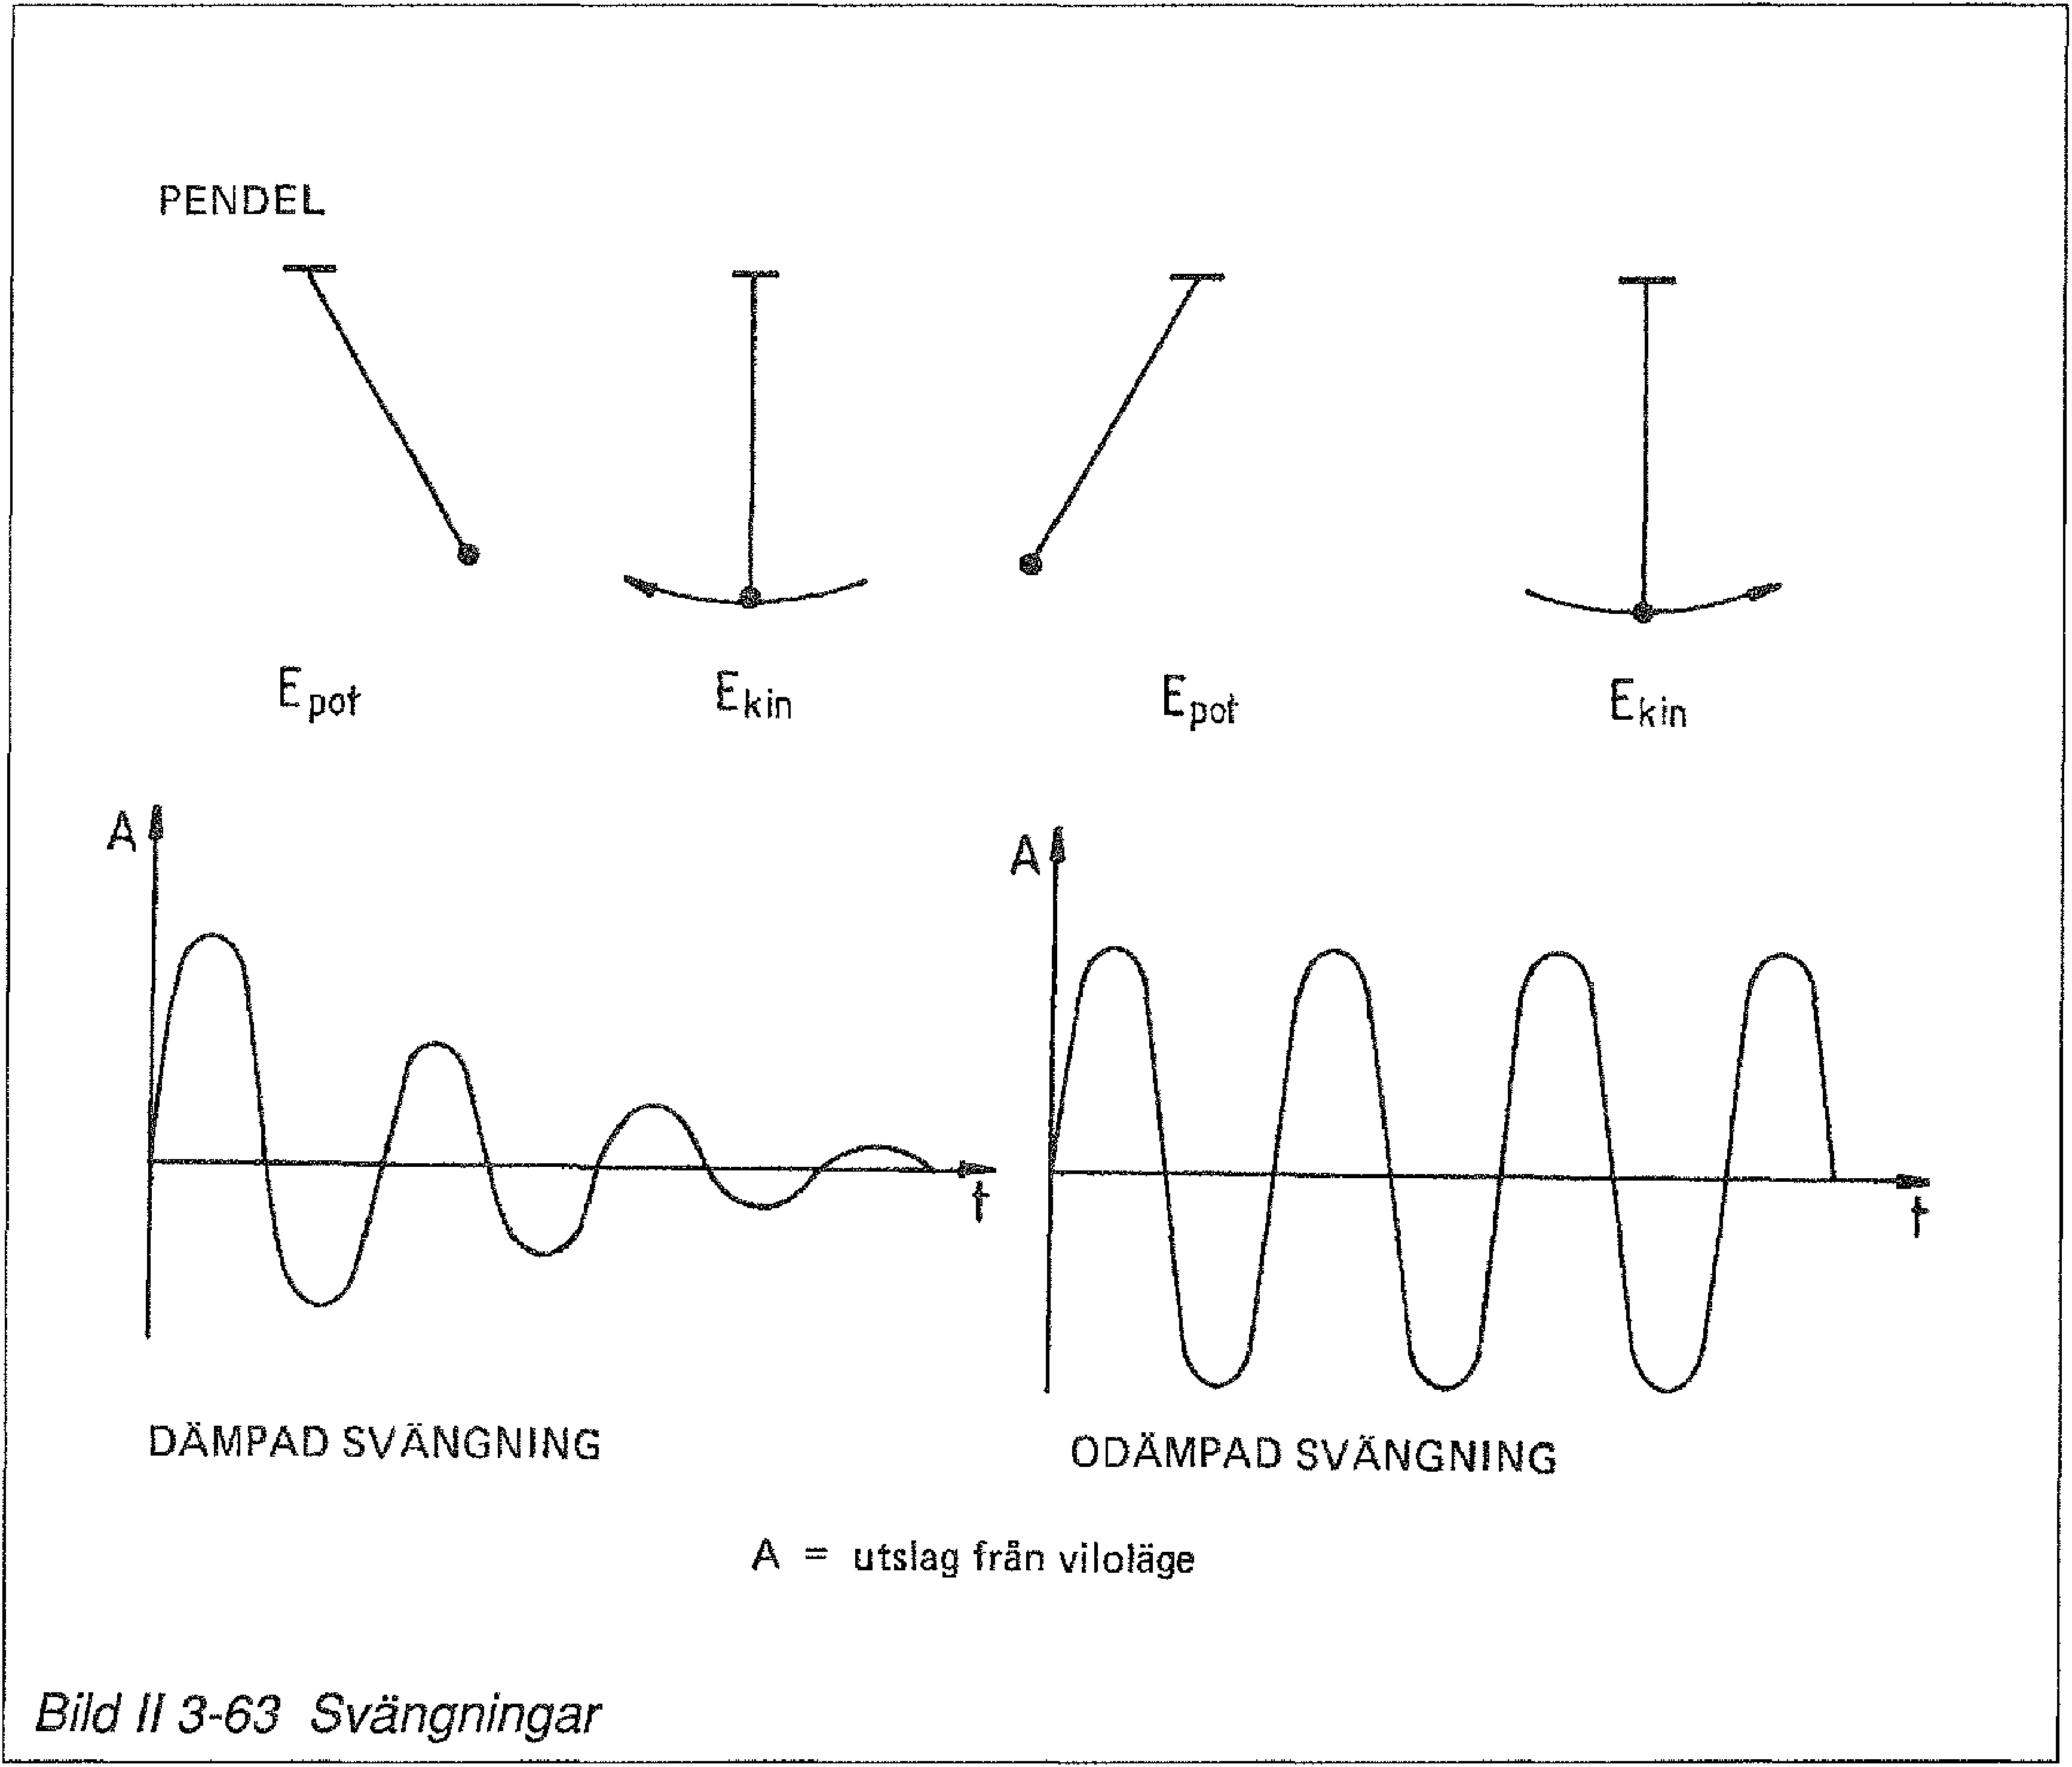
\includegraphics[width=\textwidth]{images/bild_2_3-63}
\caption{Svängingar}
\label{fig:BildII3-63}
\end{figure}

Bild \ref{fig:BildII3-63}

Energiinnehållet i en pendel växlar mellan lägesenergi (potentiell
energi) och rörelseenergi (kinetisk energi). Lägesenergin är störst i
pendelns ytterlägen och minst i mittläget. Omvänt är rörelseenergin
störst i mittläget och minst i ytterlägena.

Stöt till en pendel bara en gång så att den börjar pendla, men
utslagen blir allt mindre. Pendeln utför en dämpad svängning därför
att det förbrukas energi under pendlingen.

Dämpningen kommer av att energi förloras av friktionen i
upphängningspunkten och av luftmotståndet.

Stöt nu till pendeln varje gång, som den pendlar tillbaka. För lika
stora utslag varje gång - en odämpad svängning - fordras det upprepade
energitillskott som precis kompenserar förlusterna.

Villkoren för att en svängning ska fortgå (vara odämpad) är att
energitillskotten
\begin{itemize}
\item kommer vid rätt tidpunkt,
\item har rätt riktning- polaritet,
\item kompenserar förlusterna.
\end{itemize}

\subsubsection{Alstring av mekaniska svängningar}

\begin{wrapfigure}{R}{0.5\textwidth}
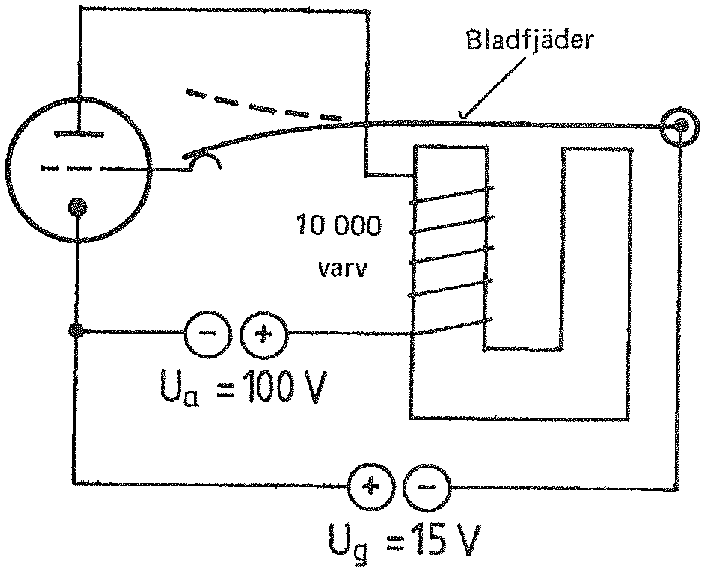
\includegraphics[width=0.5\textwidth]{images/bild_2_3-64}
\caption{Elektromekanisk oscillator}
\label{fig:BildII3-64}
\end{wrapfigure}

Bild \ref{fig:BildII3-64}

En elektrisk ringklocka med självbrytande kontakt är ett exempel på en
enkel elektromekanisk oscillator. Denna bild visar hur kontakten
ersatts med ett elektronrör. En mer ''tidsenlig'' lösning med transistor
hade naturligtvis också kunnat användas.

När anodspänningen kopplas till, så börjar anodström att flyta genom
trioden från katod till anod och genom elektromagneten.  Magneten drar
då till sig bladfjädern, som kopplar styrgallret till en negativ
förspänning.

Den negativa förspänningen stryper anodströmmen och magnetfältet
upphör. Bladfjädern släpper då från magneten och kopplar bort
styrgallret från förspänningen. Anodström börjat att flyta igen,
varvid elektromagneten drar till sig bladfjädern o.s.v. Förloppet
kallas självsvängning.

Anordningen som alstrar svängningarna kallas generator eller
oscillator. Frekvensen är det antal svängningar per sekund som
oscillatorn alstrar, i detta exempel bladfjäderns svängningshastighet.

\subsubsection{Alstring av elektriska svängningar}

\begin{wrapfigure}{R}{0.5\textwidth}
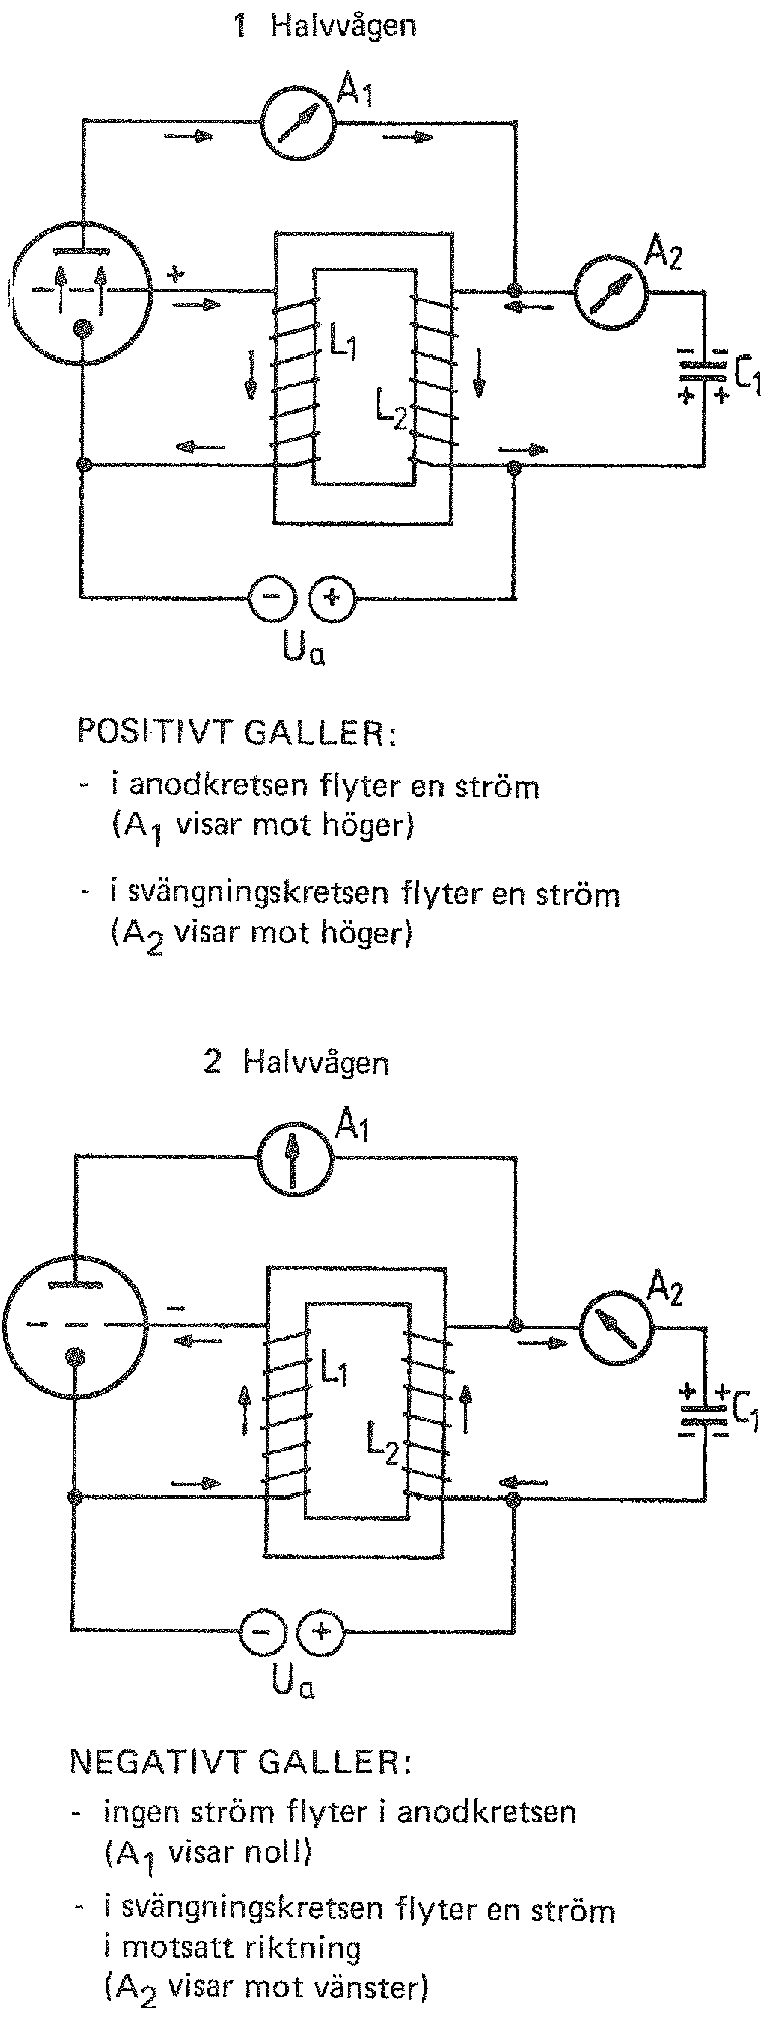
\includegraphics[width=0.5\textwidth]{images/bild_2_3-65}
\caption{Elektronisk oscillator (Meissner)}
\label{fig:BildII3-65}
\end{wrapfigure}

Bild \ref{fig:BildII3-65}

En elektrisk svängningskrets är motsvarigheten till ett mekaniskt
föremål i svängning.  Bilden visar en elektronisk oscillator med en
LC-krets i anodkretsen till en triod och som är induktivt återkopplad
till styrgallret

Amperemetern \(A_1\) visar den pulserande anodströmmen, som är en
likström. Amperemetern \(A_2\) visar växelströmmen svängningskretsen.

En elektronisk oscillator är en förstärkare, vars utsignal återförs
till ingången så att förstärkaren råkar i självsvängning - det blir en
s.k. positiv återkoppling.

Elektroniska oscillatorer används både i mottagare och
sändare. Funktionsprincipen är lika i båda fallen. Vad som möjligen
skiljer är användningssättet Det finns många oscillatorkopplingar
varav några beskrivs här.

Självsvängning kan demonstreras akustiskt med en mikrofon, en
förstärkare och en högtalare. Resultatet blir att det genereras en
ton. Ljudet från högtalaren är tryckvågor som påverkar mikrofonen och
omvandlas där till elektriska signaler. Dessa går genom förstärkaren
tillbaka till högtalaren och omvandlas åter till tryckvågor som
mikrofonen uppfattar o.s.v. Det uppstår självsvängning, ett tjut, som
beror på akustisk återkoppling.  Om förstärkaren kompletteras med ett
frekvensfilter i form av en svängningskrets, så blir ''tjutet'' i
stället en ton med samma frekvens som filtrets resonansfrekvens.

\subsection{LC-oscillatorer}
\textbf{HAREC a.\ref{HAREC.a.3.6.1}, a.\ref{HAREC.a.3.6.2}, a.\ref{HAREC.a.3.6.3}\label{myHAREC.a.3.6.1}\label{myHAREC.a.3.6.2}\label{myHAREC.a.3.6.3}}
\index{LC-oscillator}
\index{oscillator!LC}

\subsubsection{Variabel frekvens oscillator - VFO}
\index{oscillator!VFO}
\index{oscillator!variable frekvens}

\begin{wrapfigure}[32]{R}{0.5\textwidth}
  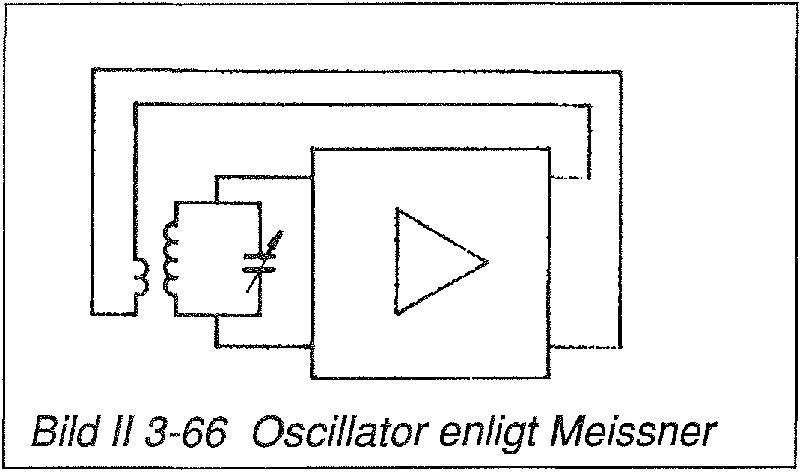
\includegraphics[width=0.5\textwidth]{images/bild_2_3-66}
  \caption{Oscillator enligt Meissner}
  \label{fig:BildII3-66}

  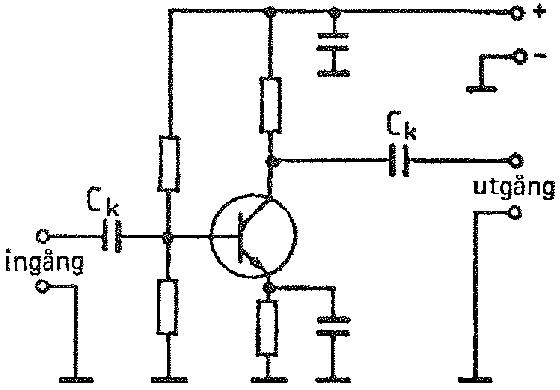
\includegraphics[width=0.5\textwidth]{images/bild_2_3-67}
  \caption{Emitterkopplad förstärkare}
  \label{fig:BildII3-67}

  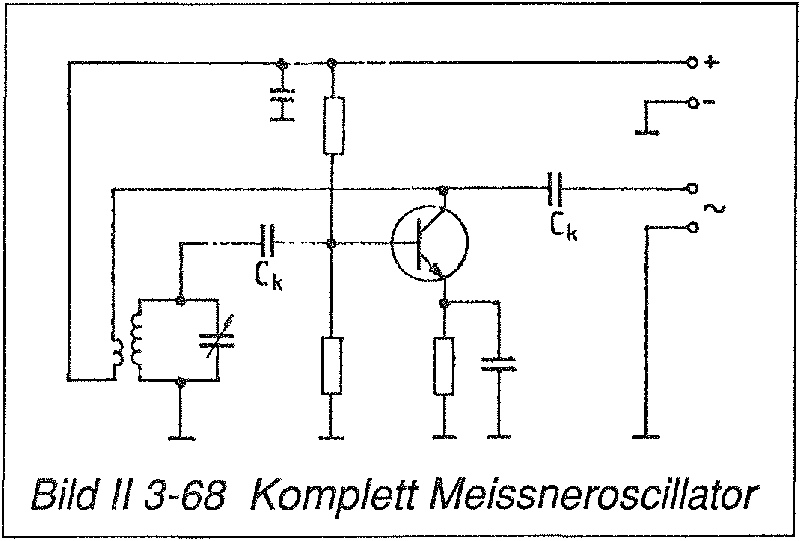
\includegraphics[width=0.5\textwidth]{images/bild_2_3-68}
  \caption{Komplett Meissneroscillator}
  \label{fig:BildII3-68}
\end{wrapfigure}

En oscillator med inställbar frekvens kallas för VFO (variabel
frekvensoscillator). Förutom frekvensstabilitet fordras också, att
noggrann inställning och avläsning av frekvensen ska kunna göras.

En LC-oscillator är urtypen för en oscillator med variabel
frekvens. Meissner-kopplingen är lätt att urskilja och används här för
att beskriva grundprincipen för en oscillator i stort. Bl.a. Colpitts-
och Clapp-kopplingarna har emellertid bättre stabilitet och
inställbarhet i återkopplingsledet

\subsubsection{Meissner-koppling}
\index{Meissner-koppling}
\index{oscillator!Meissner-koppling}

Bild \ref{fig:BildII3-66}

Bilden visar en Meissner-oscillator, som består av en
LC-svängningskrets med återkopplingsspole och en
förstärkare. Magnetfältet mellan induktansen i svängningskretsen och
återkopplingsspolen är polariserat så att en förändring i utsignalen
medverkar till självsvängning. (Motsatsen är motkoppling.)

Bild \ref{fig:BildII3-67}

Förstärkaren kan t.ex. vara en emitterkopplad transistorförstärkare
enligt bilden.  Kopplingskondensatorerna \(C_k\) är nödvändiga för att
förhindra kortslutning av de likspänningar som pestämmer arbetspunkten
för transistorn. Å andra sidan kan växelspänningssignalerna passera
till och från transistorn.

Bild \ref{fig:BildII3-68}

Återkopplingsvägen görs i detta fall så, att svängningskretsen kopplas
parallellt över förstärkaringången. Återkopplingsspolen fungerar som
förstärkarens kollektorresistor.

\subsection{Självsvängningsvillkoret}
\index{oscillator!självsvängningsvillkoret}

\begin{wrapfigure}{R}{0.5\textwidth}
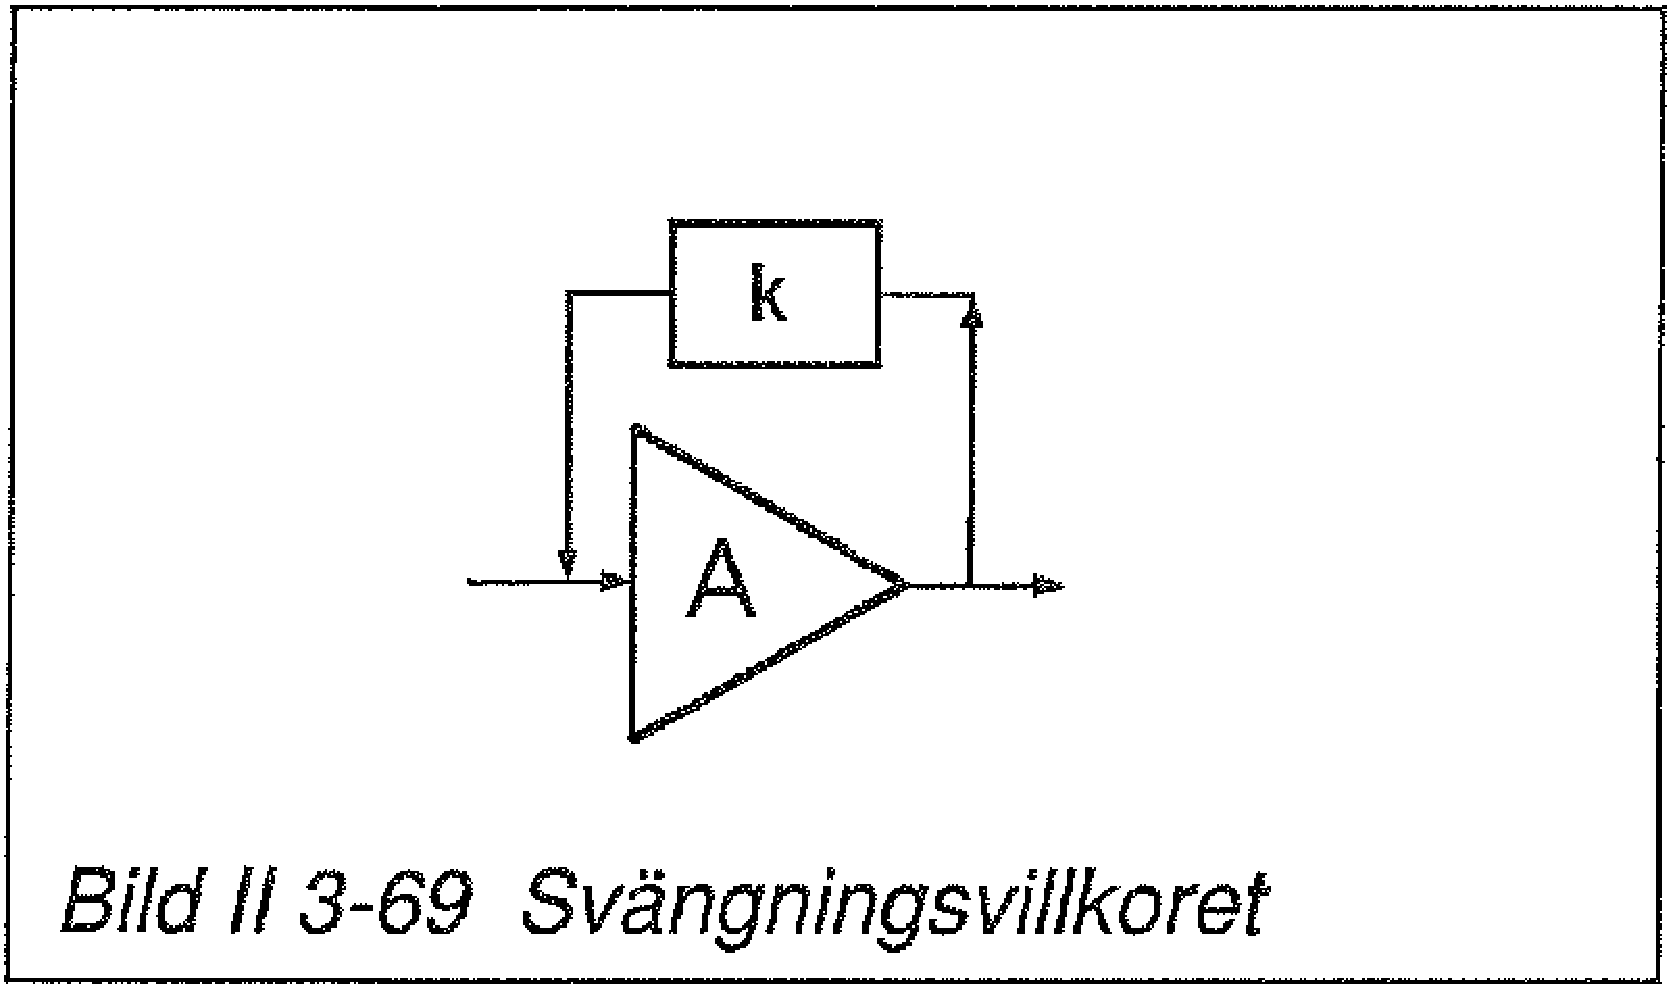
\includegraphics[width=0.5\textwidth]{images/bild_2_3-69}
\caption{Svängningsvillkoret}
\label{fig:BildII3-69}
\end{wrapfigure}

Bild \ref{fig:BildII3-69}

Självsvängning i en förstärkare uppstår genom
återkoppling. Signalspänningen \(\hat{U}_{in}\) över ingången blir
förstärkt med faktorn \(A\). När som i bild II 3-68 förstärkaren är
emitterkopplad, blir utsignalen fasvriden 180° i förhållande till
insignalen. Fasvridningen \(\alpha=180°\) betecknas här med
minustecken, alltså blir förstärkningen \(-A\).

På förstärkarens utgång fås en signalspänning \(\hat{U}_{ut}\) med
sambandet

\[\hat{U}_{ut} = -A \cdot \hat{U}_{in}\]

En del av utsignalen återförs (återkopplas) till ingången. I en
Meissner-oscillator sker återkopplingen med en induktor, som är
induktivt kopplad till svängningskretsens induktor.

Kvoten \(k\) mellan den återkopplade signalspänningen \(\hat{U}_{ut}\) och
signalspänningen out på förstärkarens utgång kallas
återkopplingsfaktor. Den återkopplade spänningen \(\hat{U}_k\) fasvrids så
att den kommer ''i fas med'' med insignalen. För den återkopplade
signalen fås då sambandet

\[\hat{U}_k = -k \cdot \hat{U}_{ut}\]

Tillräcklig signalspänning från utgången måste återföras till ingången
för att det ska uppstå självsvängning. Det sker när den återkopplade
signalspänningen \(\hat{U}_k\) är minst lika stor som
ingångsspänningen \(\hat{U}_{in}\) och är i rätt fasläge, d.v.s. i
detta exempel

\[
\hat{U}_k \geq \hat{U}_{in}
\quad \text{eller} \quad
-k \cdot \frac{\hat{U}_{ut}}{A}
\quad \text{eller} \quad
k \geq \frac{1}{A}
\]

Självsvängningsvillkoret blir

\[
k \geq \frac{1}{A}
\quad \text{eller} \quad
k \cdot A \geq 1
\]

Ett \(k \cdot A \approx 3\) är önskvärt för att oscillatorn ska
svänga igång snabbt.

\subsubsection{Hartley-koppling}
\index{Hartley-koppling}
\index{oscillator!Hartley-koppling}
\index{Huth-Kügn-koppling}
\index{oscillator!Huth-Kügn-koppling}
\index{Tuned Grid Tuned Plate-koppling}
\index{oscillator!Tuned Grid Tuned Plate-koppling}

\begin{wrapfigure}[25]{R}{0.5\textwidth}
  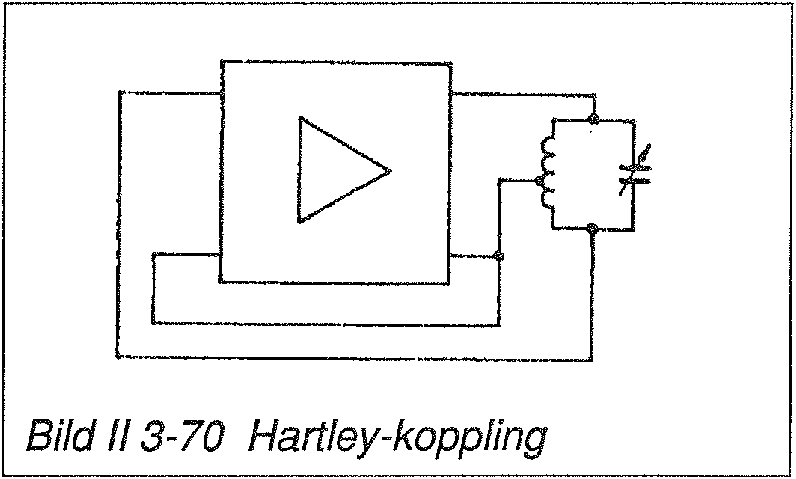
\includegraphics[width=0.5\textwidth]{images/bild_2_3-70}
  \caption{Hartley-koppling}
  \label{fig:BildII3-70}

  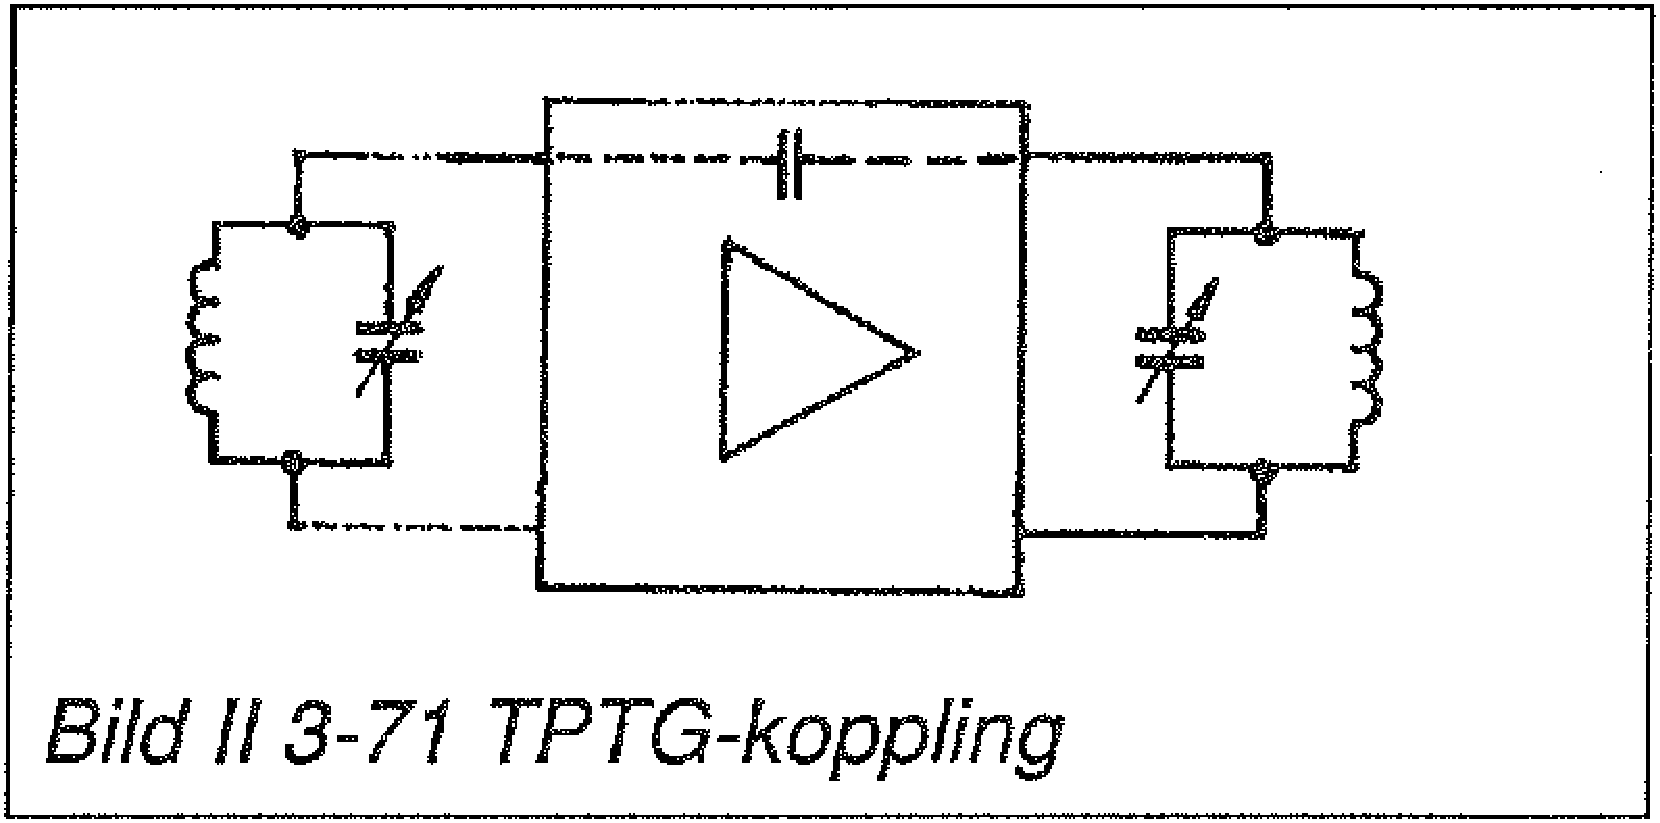
\includegraphics[width=0.5\textwidth]{images/bild_2_3-71}
  \caption{TPTG-koppling}
  \label{fig:BildII3-71}

  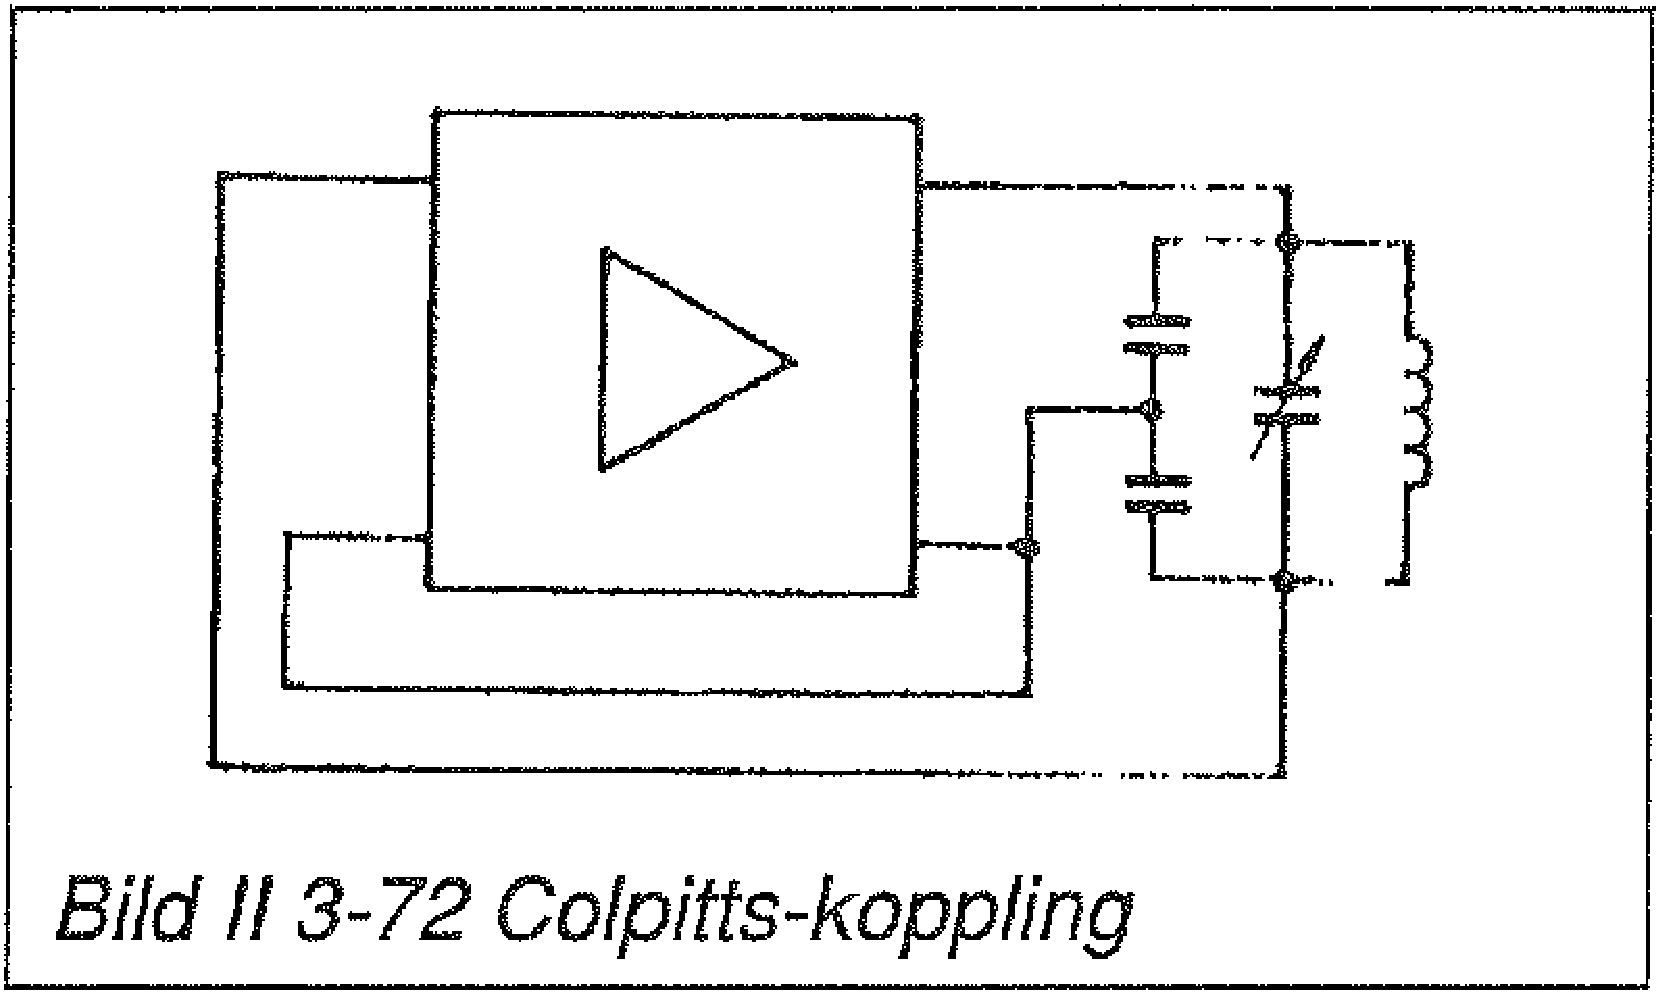
\includegraphics[width=0.5\textwidth]{images/bild_2_3-72}
  \caption{Colpitts-koppling}
  \label{fig:BildII3-72}
\end{wrapfigure}

Bild \ref{fig:BildII3-70}

Återkopplingen sker galvaniskt över ett uttag på induktorn i
oscillatorns LC-krets.

Huth-Kühn eller TGTP-koppling (tuned grid - tuned plate)

Bild \ref{fig:BildII3-71}

Kopplingen är en förstärkare med LC-kretsar både på in- och
utgång. Båda kretsarna är avstämda till samma frekvens. Återkopplingen
sker över de inre kapacitanserna mellan elektronrörets elektroder
resp. mellan transistorns materialskikt Denna koppling är av flera
skäl inte särskilt vanlig.

\subsubsection{Colpitts-koppling}
\index{Colpitt-koppling}
\index{oscillator!Colpitt-koppling}

Bild \ref{fig:BildII3-72}

Återkopplingen sker över en kapacitiv spänningsdelare, som ingår som
en del av oscillatorns LC-krets.

\subsubsection{Clapp-koppling}
\index{Clapp-koppling}
\index{oscillator!Clapp-koppling}

Denna koppling är en variant av Colpitts-kopplingen. Vridkondensatorn
för frekvensinställningen är seriekopplad med spänningsdelarens
kondensatorer. Clapp-oscillatorns frekvensstabilitet är god.

Bild \ref{fig:BildII3-73a}

Vi utvecklar denna beskrivning vidare.  Vridkondensatorn samt en fast
och en trimningsbar kondensator är kopplade parallellt med
varandra. Alla tre kondensatorerna är i sin tur seriekopplade med den
kapacitiva spänningsdelaren \(C_3\) / \(C_4\).  Förstärkarens ingång
är kopplad till den övre anslutningen av \(C_3\). Utgången från
oscillatorns förstärkare återkopplas över dämpresistorn Rct till
mitten av spänningsdelaren \(C_3\) / \(C_4\) (återkopplingskretsen).

Bild \ref{fig:BildII3-73b}

Förstärkarens arbetspunkt bestäms av spänningsdelaren \(R_1\) /
\(R_2\). Ingen kopplingskondensator behövs eftersom det enbart finns
kondensatorer mellan förstärkaringång och jord.  Kondensatorn \(C_6\)
avkopplar kollektorn på transistor \(T_1\) HF-mässigt till
jord. Förstärkaren är alltså kollektorkopplad.

Kondensatorn \(C_7\) kopplar oscillatorns utsignal till buffertsteget
För frekvensstabilitetens skull stabiliseras spänningen 8 V med en
lC-krets som avkopplas HF-mässigt med en kondensator.

\subsection{Frekvensinställning och bandspridning}
\index{oscillator!frekvensinställning}
\index{oscillator!bandspridning}

\begin{wrapfigure}{R}{0.5\textwidth}
  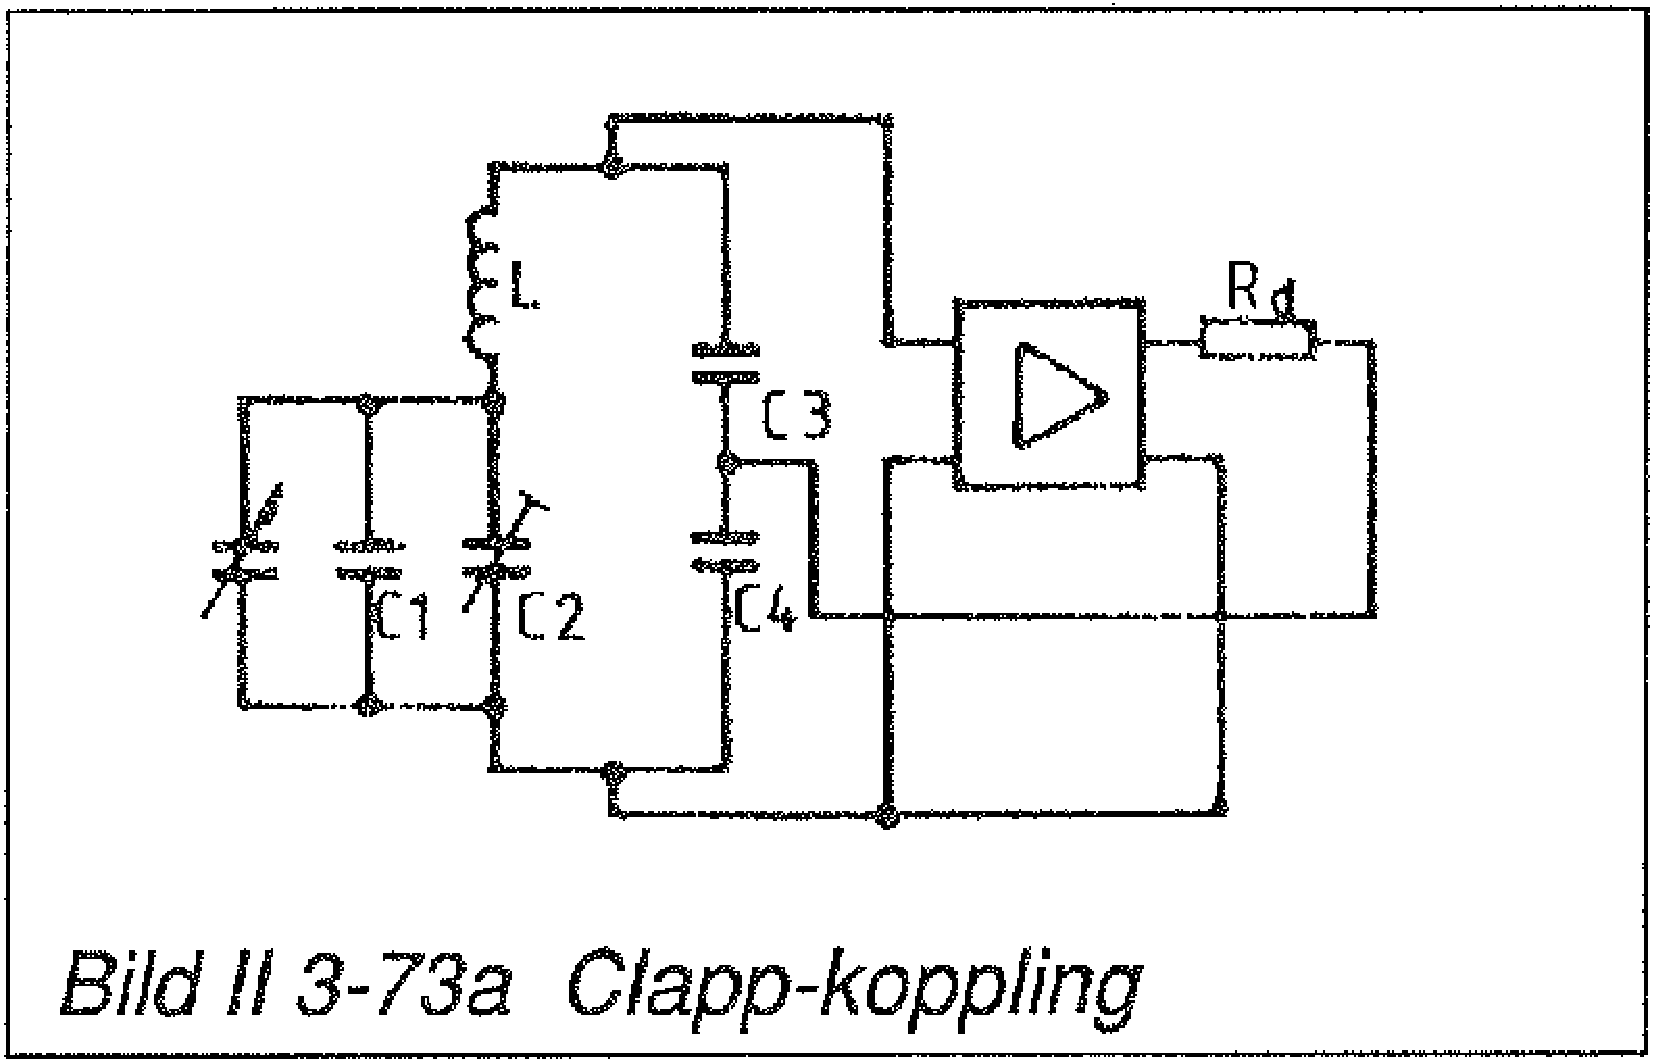
\includegraphics[width=0.5\textwidth]{images/bild_2_3-73a}
  \caption{Clapp-koppling}
  \label{fig:BildII3-73a}

  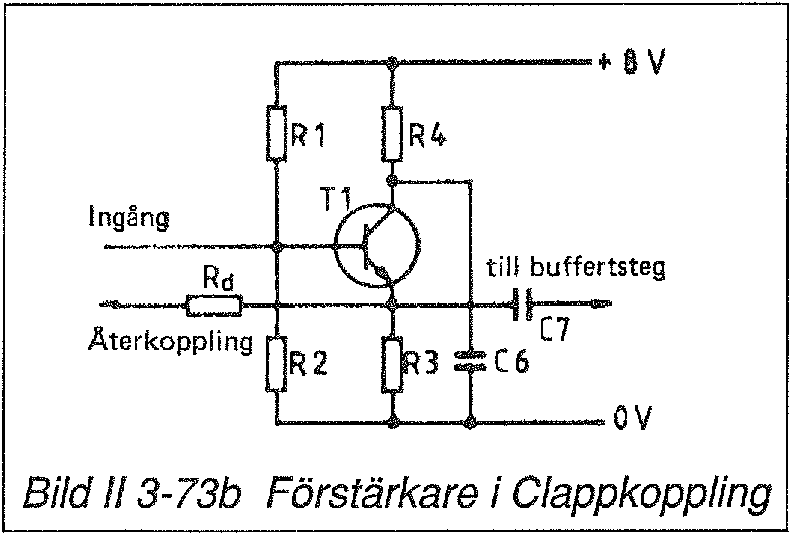
\includegraphics[width=0.5\textwidth]{images/bild_2_3-73b}
  \caption{Förstärkare i Clappkoppling}
  \label{fig:BildII3-73b}

  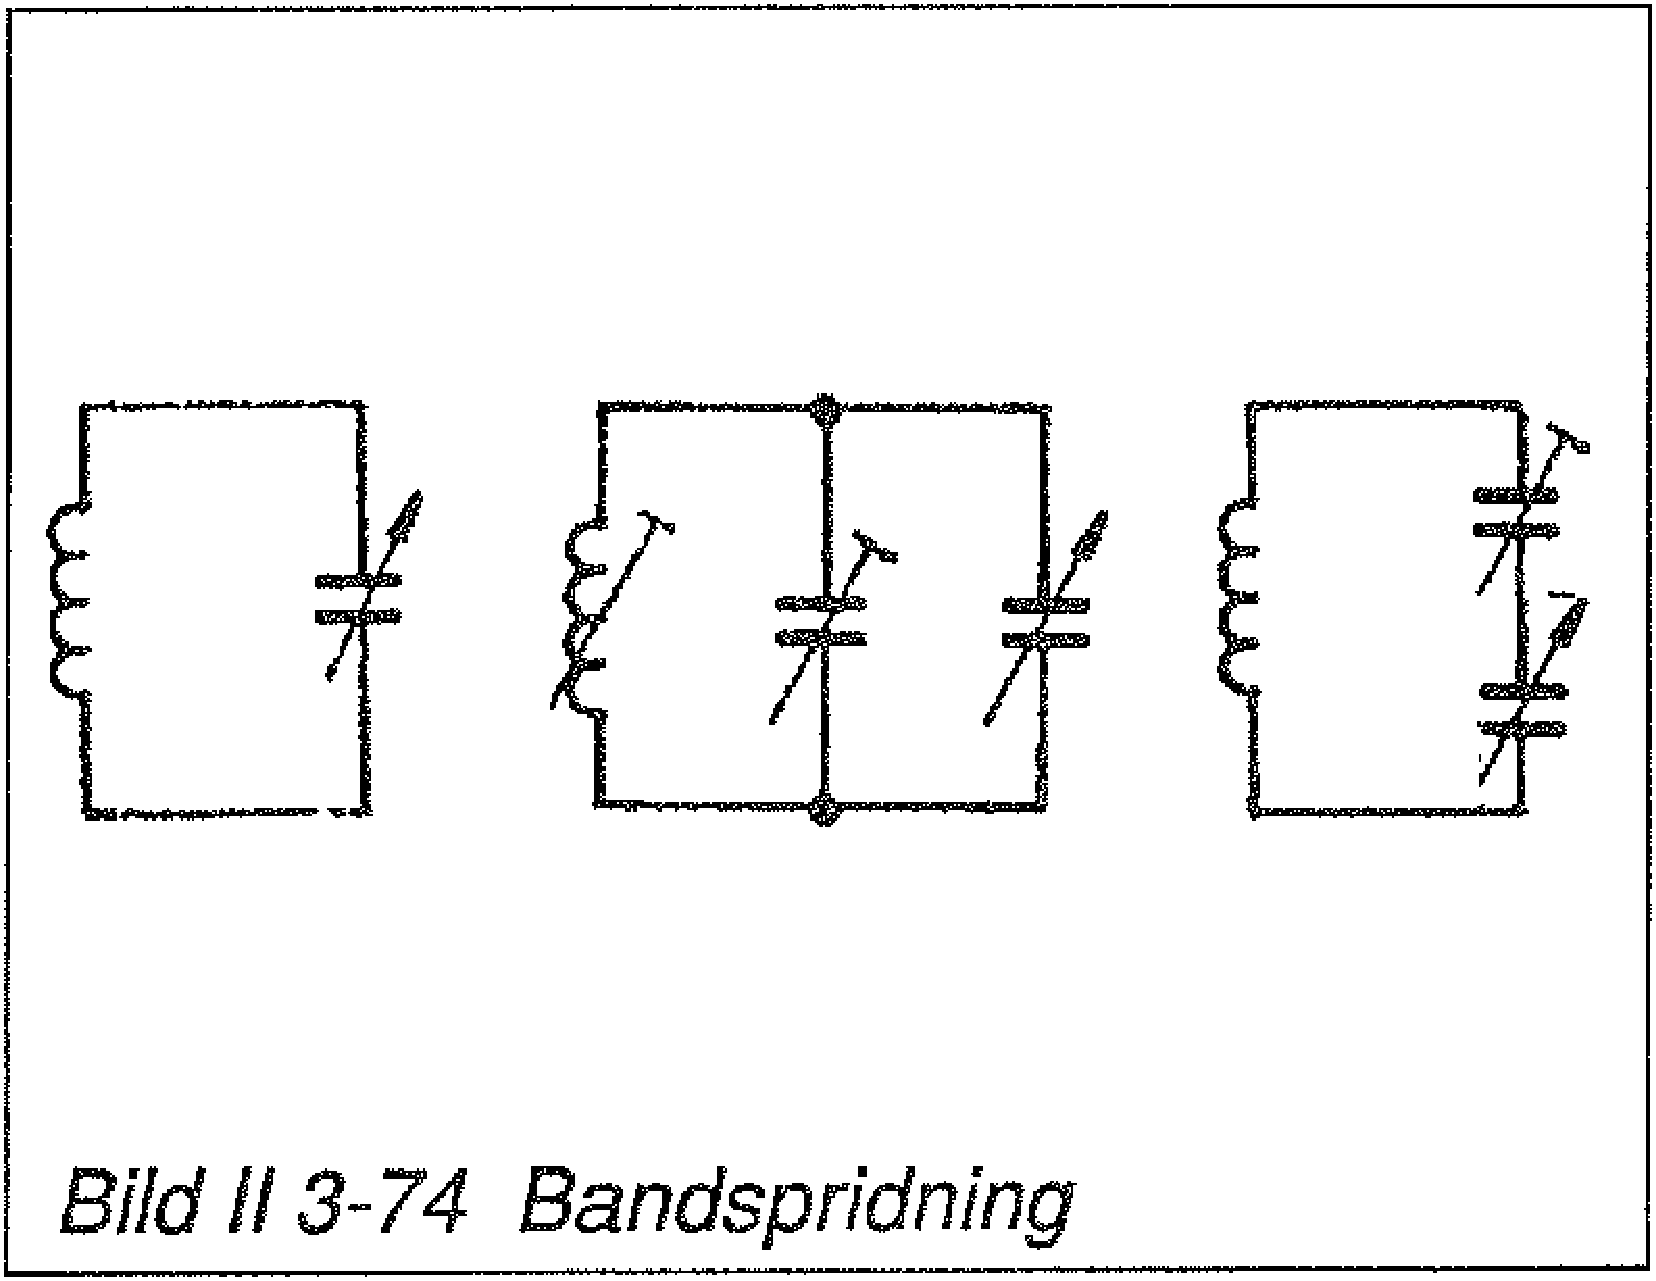
\includegraphics[width=0.5\textwidth]{images/bild_2_3-74}
  \caption{Bandspridning}
  \label{fig:BildII3-74}
\end{wrapfigure}

Bild \ref{fig:BildII3-74}

Att ställa in frekvensen i en LC-oscillator gjordes förr oftast med en
vridkondensator. I moderna mottagare och sändare används i stället en
s.k. varicap, som styrs med en likspänning.

Med en svängningskrets med endast en induktor och en vridkondensator,
skulle alla amatörradiobanden endast vara smala områden utspridda på
en mekanisk skala, d.v.s.  över vridkondensatorns hela
kapacitansområde, varvid kapacitansen kan varieras med förhållandet
1:5 à 1:10, t.ex. 10-50~pF à 10-100~pF.

För att i stället få vart och ett av amatörradiobanden utspridda över
större delen av skalan kan man ordna med bandomkoppling och
s.k. bandspridning. Man parallellkopplar då en relativt stor fast
kapacitans med vridkondensatorns relativt lilla kapacitans. Den totala
kapacitansvariationen i LC-kretsen blir då liten, trots att
kondensatorns hela kapacitansområde utnyttjas. Resultatet blir en
frekvensskala med större upplösning, d.v.s. bättre
avläsningsnoggrannhet.

Bandspridning kan också ordnas med två seriekopplade kondensatorer,
varav den större görs variabel. Typiskt värde på vridkondensatorn i en
kortvågsutrustning är då 100--500~pF och den fasta kondensatorn mycket
mindre än så.
